


\section{Common Spatial Patternとその派生手法}
運動想起型BCIに対しては``Common Spatial Pattern(CSP)''\cite{csp}が1999年に提案されて以降、
非常に活発に応用研究がされている。その後、ベンチマークとして引用されてきただけでなく、
CSPの拡張手法も数多く提案されてきた。
CSPは脳波解析の分野で発展した手法であるため、その定式化も脳波計測時のデータ構造に合わせた
形式となっている。そのため、今一度脳波信号の定式化を述べた後にCSPについて記す。

\subsection{脳波信号の定式化}
これまで多次元の信号を\(x(t)\in \mathbb R^D\)と表記し、連続時間信号として扱ってきた。
しかし、通常は計測された脳波はコンピュータで処理するために
離散時間信号\(x_n \in \mathbb R^D\)に変換される。
従って、以降、脳波信号を離散時間信号として取り扱う。
また、運動想起時の脳波信号を計測する際には、
被験者に対して定められたタイムスケジュールで運動想起を行うように指示がなされる。
例として64個の電極を用い、サンプリング周波数100Hzで10秒間の計測を行った場合、
計測された運動想起1回分の脳波信号は\(X \in \mathbb{R}^{64 \times 1000}\)
と表すことができる。従って、以降統一のため、\(M\)を電極の個数、
\(N\)を計測時間点数とした場合の脳波信号を以下で定義する\begin{equation}
    X =(x_1, \cdots, x_N)\in \mathbb{R}^{M \times N}\    
\end{equation}。


運動想起を\(K\)回行った場合には、\(K\)個の\(X\)が得られる。
通常は運動想起時の脳波を数個から数十個集め、統計的な指標を元に有用な特徴量を抽出する。
CSPは運動想起BCIに対して極めて有効に働くとされている特徴量抽出手法である。


\subsection{Common Spatial Pattern(CSP)}
\label{subsec:CSP}

CSPを脳波に用いる際は、脳波信号\(X\)を直接扱うのではなく、何らかの前処理を施した信号\(\hat{X} = {\cal H}(X) \)を用いる。
通常、\(\cal H\)には、運動想起に関連のある周波数帯域のみを通過させるバンドパスフィルタを用いる。
バンドパスフィルタ通過後の脳波信号を以下のように表記する。
\begin{equation}
    \hat X = \left( \hat x_1,\cdots,\hat x_N \right) \in \mathbb{R}^{M \times N}
\end{equation}
\(\hat x_i \in \mathbb R^M\)における添字\(i\)はサンプル時刻の添え字である。
CSPでは、新たな基底\(w\in \mathbb R^M\)にバンドパスフィルタ通過後の脳波信号を射影し、
スカラー時間信号である\(z=w^T\hat X\in \mathbb R^N\)を抽出する。この時の\(w\)の決め方を以下に記す。

まず\(\hat X\)を基底\(w\)に射影した際の時間分散\(\sigma^2 (\hat X, w)\)を以下で定義する。
\begin{equation}
    \sigma^2 (\hat X, w)  = \frac{1}{N}\sum_{i=1}^N \left|w^T \left(\hat x_i - \frac{1}{N} \sum_{j=1}^N \hat x_j \right) \right|^2
    \label{timevar}
\end{equation}
ここで計測された複数個の\(\hat X\)は必ず集合\(C_1\)か\(C_2\)のいずれか一方に属するとし、
\(C_1 \cap C_2 = \phi \)であるとする。
CSPでは、ベクトル\(w \in \mathbb {R}^M\)を新たな基底とした電極空間において、
一方のクラスに属する信号\(\hat X \in {C_d}\)についての時間分散(\ref{timevar})が最大となるように、\(w\)を決める。
これは以下の最大化問題によって定式化される。
\begin{equation}
    \begin{aligned}
    & \max_w
    & & \mathbb E_{X \in C_1} \left[\sigma^2 (\hat X, w) \right] \\
    & \text{s.t.}
    & &  \sum_{d=1,2} \mathbb E_{X \in C_d} \left[\sigma^2 (\hat X, w) \right] = 1
    \end{aligned}
    \label{objcsp}
\end{equation}

最大化問題(\ref{objcsp})を解いて得られる\(w\)は、
クラス\(C_1\)に属する脳波の振幅を最大化するような基底となっている。
一方で、制約条件によってクラス\(C_2\)に属する脳波の振幅を最小化する基底ともなっている。
この最適化問題の解法はよく知られており、標準的な解法は一般化固有値問題を解くことと等価である。計算量の観点から効率の良い解法も提案されている。固有値が分散に、固有ベクトルが新しい基底に対応し、
最大固有値に属する固有ベクトルと、最小固有値に属する固有ベクトルを新たな基底として用いる。
通常は変換先での時間分散の対数値を特徴量として用いる。以下の図はトイデータを使ったCSPによる特徴量抽出の様子である。

\begin{figure}
    \centering
    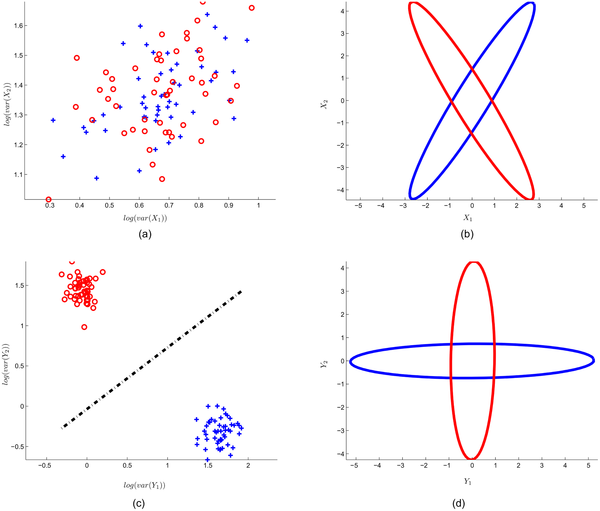
\includegraphics[width=12cm]{images/apple.png}
    \caption{林檎の図}
\end{figure}
  

\subsection{Common Spatiospectral Pattern(CSSSP)}
CSPではバンドパスフィルタ\(\cal H\)通過後の信号を扱ったため、バンドパスフィルタの設計を終えてからでなければCSPの問題を解くことができない。
しかし、バンドパスフィルタの設計次第ではCSPの解が変わることが想定される。そこで、バンドパスフィルタの設計をCSPの問題の中に取り込んだのがCSSSP\cite{csssp}である。

まず脳波信号\(X = \left[ x_1, \cdots, x_N \right] \in \mathbb{R}^{M \times N}\)に対して、
観測時間点を\(\tau\ > 0\)だけずらした\(X_{\tau} = \left[ x_{1+\tau}, \cdots, x_{N+\tau} \right] \in \mathbb{R}^{M \times N}\)を考える。
ここで$\tau = 1,\ldots,T$であり、$T$がFIRフィルタの次数の役割を担う。
更にクラス\( C_d \)に属する\( X \)に関して、
\begin{equation}
    \Sigma_{d}^{\tau} = \mathbb E_{X \in C_d} \left[ XX_{\tau}^T + X_{\tau}X^T \right]
\end{equation}
を定義する。ただし、\( \Sigma_{d}^{0} = \mathbb E_{X \in C_d} \left[XX^T \right] \)とする。FIRフィルタの実数係数ベクトルを$b=[1,b_2,\ldots,b_T]^T$として、
CSSSPの最適化問題は以下で表現される。
\begin{equation}
    \begin{aligned}
    & \max_{b_2,\ldots,b_T} \max_{w}
    & & w^T \left\{ \sum_{\tau = 0}^{T-1} \left( \sum_{j=1}^{T-\tau} b_j b_{j+\tau} \right) \Sigma_1^{\tau} \right\} w - \frac{\alpha}{T}|b|_1 \\
    & \text{subject to}
    & &  w^T \left[\sum_{\tau = 0}^{T-1} \left\{ \sum_{j=1}^{T-\tau}b_jb_{j+\tau} \right\} (\Sigma_1^{\tau} + \Sigma_2^{\tau}) \right] w = 1
    \end{aligned}
\end{equation}
この最適化問題では空間重みベクトル\(w \in \mathbb R^M\)とFIRフィルタの実数係数ベクトル$b$を同時に評価することが可能である。
目的関数における第二項は正則化項であり、$\alpha$はハイパーパラメータである。
この正則化によってFIRフィルタの系列ベクトルに対してスパース性が要請され、FIRフィルタが異常に複雑になることが避けられる。


\subsection{Filter Bank Common Spatial Pattern(FBCSP)}
CSSSPはFIRフィルタの設計をCSPの最適化問題に含むことで、バンドパスフィルタとCSPの同時最適化の定式化に成功した。
しかし、CSSSPによって求まる特徴量は1つのFIRフィルタを通過し、1つのCSPによって電極の重み付けが行われた脳波信号にすぎない。
クラス分類を行うことが最終目標であることを考えれば、この特徴量は必ずしも最適なものであるとは言い難い。
例えば左手の運動想起時と下肢の運動想起時では重要な周波数帯域が異なるためである。すなわちCSSSPによって決定されたFIRフィルタは、
左手の運動想起時に重要な周波数帯域を捉えている一方で、下肢に重要な帯域を失ってしまっているということが生じうる。FBCSPはこのような問題の解決を図る手法である。

まず、バンドパスフィルタバンク\(\{ {\cal H}_1, \ldots, {\cal H}_F \}\)を定義する。
各バンドパスフィルタを通過した\(\hat X_f = {\cal H}_f(X)\)に対して、それぞれCSPの問題を解くことで、複数の周波数帯域を反映した特徴量の抽出が可能となる。
しかし、この段階においてはCSSSPとは異なり、CSPとバンドパスフィルタの同時最適化を行ってはいないため、初めに定義したバンドパスフィルタバンクのCSP特徴量を対等に扱うことが妥当とは言えない。
FBCSPでは各バンドパスフィルタに対してのCSPの解から、
更に重要な特徴量の選定を行う方法までを含んだ提案がなされている\cite{fbcsp}。